\setchapterpreamble[u]{\margintoc}
\chapter{Integration in a Proof Assistant}
\labch{plugin}

In the previous chapters, we introduced the Proof-by-Action paradigm
(\refch{pba}), and tried to convince the reader that it is both theoretically
sound with its firm grounding in deep inference proof theory (\refch{sfl} and
\refch{sfl-classical}), and practically useful by analysing proofs of
mathematical problems expressed within it (\refch{advanced}). We also mentioned
multiple times our prototype of interface implementing Proof-by-Action called
Actema, and in particular the fact that it exists as a \emph{standalone} web
application with its own proof engine \sidecite[5em]{Actema:link}. This is
convenient for distributing it online as a publicly available website, so that
people can immediately try it out without the hassles of installation
procedures. However due to both historical choices in its design and lack of
human resources for development, Actema's proof engine is quite limited in its
features:
\begin{itemize}
  \item it can only handle goals expressed in many-sorted intuitionistic
    first-order logic (hereafter iFOL), whereas all state-of-the-art PAs support
    \emph{higher-order logic} in one form or another; and higher-order features
    are crucial for formalizing many mathematical notions in a concise way, as
    witnessed by the example of \refsec{funcs};
  \item it does not implement a \emph{certified logical kernel} for checking proof
    objects, which makes it hard to trust and interoperate with;
  \item it has no mechanism for adding new \emph{mathematical notations}, only
    ad hoc support for arithmetical expressions; thus formulas become very
    quickly impossible to read and manipulate;
  \item it has poor support for managing \emph{libraries} of definitions, lemmas
    and proofs, partly because of the previous items.
\end{itemize}
% Typically, the example studied in \refsec{funcs} cannot be carried out in the
% standalone version of Actema, because it lacks support for defining new
% predicates --- especially when they are higher-order like $\injective(\cdot)$
% --- as well as new notations for them like $\subseteq$ for set inclusion.

To address these limitations, and thus enable a confrontation of the
Proof-by-Action paradigm to real mathematical developments, we decided to build
\texttt{coq-actema}, a Coq plugin that directly connects Actema to a running
instance of the Coq PA. The idea is that Actema should act as an enhanced
graphical, interactive proof view that integrates in the usual text-based
workflow of proof scripts. Thus instead of trying to turn Actema into a
full-fledged PA, we exploit the over 30 years of effort that have been put in
the development of Coq, and limit the role of Actema to that of a novel frontend
for building proofs in Coq. This shall open the way to more advanced
experimentations through the huge body of theories already developed in Coq, and
make the Proof-by-Action paradigm visible to the large community of existing
users of this popular PA.

Note that the same approach should be applicable in principle to any ITP that
supports at least iFOL, and provides an interaction protocol for building proofs
in a goal-directed manner. This includes other popular PAs such as Lean and
Isabelle, but also more specialized software like the Why3 platform for
deductive program verification, the Meta-F* framework in the F* programming
language, or the EasyCrypt toolset for proving cryptographic protocols\todo{add
citations}.

% Moreover, since Actema works with goals expressed in iFOL, the same approach
% could be applied to any goal-directed ITP whose logical framework supports iFOL,
% which is virtually every ITP.

The chapter is organized as follows: we start in \refsec{actema} by explaining
the implementation design of the Actema web application, which follows the
standard conceptual separation between frontend and backend. In
\refsec{whyplugin}, we reflect on some considerations that led us to the
specific choice of a Coq plugin, in order to integrate the Actema web app with
Coq. Then in \refsec{architecture} we present the architecture of the
\texttt{coq-actema} system, which structures all interactions between the user,
Coq and Actema. \refsec{protocol} describes in more details the main usage
scenario of \texttt{coq-actema}, following the flow of data and control between
the different processes involved. \refsec{compilation} explains how the various
graphical actions performed by the user in Actema are compiled into Coq tactics,
ultimately producing certified proof terms. Finally in \refsec{pluginfuture}, we
discuss possible avenues for extending the usability of \texttt{coq-actema} to a
broader class of Coq goals, as well as prospective solutions to the problem of
\emph{proof evolution} in our graphical paradigm.

\section{Actema}\labsec{actema}

At its core, Actema is a web application made of two components: a
\emph{frontend} that implements the graphical interface with which the user
interacts, written in HTML/CSS and JavaScript with the Vue.js framework
\sidecite{Vuejs}; and a \emph{backend} that implements the proof engine, written in
OCaml and compiled to JavaScript (JS hereafter) with js\_of\_ocaml
\sidecite{vouillon_bytecode_2014}. The two components interact through an
object-oriented API written in OCaml, which is loaded at runtime in the form of
a JS object called \texttt{engine}, and whose methods can be called from the Vue
components in the frontend.

The \texttt{engine} object provides various high-level methods for handling the
current \emph{proof state}. Common operations include getting the list of open
subgoals, querying available proof actions on a subgoal, or applying a given
proof action. Lower-level methods are also available in other objects to inspect
the data of the proof state. For instance,
$$\mathtt{engine.subgoals[0].context[0]}$$
will return an object representing the first hypothesis of the first subgoal;
and this object itself exposes an \texttt{html} method, which returns a string
holding the HTML code used to display the statement of the hypothesis.

\todo{Add a little side figure illustrating an API call to the backend? Or we
wait for the description of the sequence diagram of \refsec{protocol}.}

In the standalone version of Actema, the proof engine takes care of computing
the new subgoals stemming from actions performed by the user. It is thus
responsible for defining the \emph{semantics} of proof actions. It is also in
charge of various other tasks that process the logical data of the proof state,
typically checking the \emph{validity} of linkages during a DnD action, which
requires the use of a unification algorithm (see \refsec{validity}).

\section{Why a plugin?}\labsec{whyplugin}

Usually, integrated development environments for Coq live in an independent
process, and exchange data with Coq through a high-level communication protocol:
either the command line interface provided by \texttt{coqtop}, Coq's default XML
protocol, or its improved superset SerAPI \sidecite{gallegoarias:hal_01384408}. In
particular, SerAPI emerged from the development of jsCoq
\sidecite{Gallego_Arias_2017}, an IDE that runs entirely in web browsers by
embedding a version of Coq compiled with js\_of\_ocaml. Since Actema is also
web-based and uses js\_of\_ocaml, our first idea was essentially to fork jsCoq
and replace its interface by that of Actema. However as noted by E. J. G.
Arias\sidenote{In private communication.}, the SerAPI protocol --- and in fact
all the other protocols turn out to be too high-level for our purpose. Typically
we need to (partially) translate Coq goals into iFOL goals, which can be done
much more easily with a direct access to Coq's low-level API for manipulating
kernel terms.
% We also heavily rely on unification to interactively suggest valid
% actions on subterms of the goal, and none of the protocols implement unification
% queries.

Now, remember that Actema is not meant as a full-fledged IDE that can manage the
edition and execution states of the proof script, but only as an enhanced proof
view for manipulating already-parsed goals. One should think of Actema's actions
as just a graphical frontend for invoking a new set of tactics. And this is
precisely what the plugin system of Coq has been designed for: extending Coq
with new tactics. Thus the solution of a Coq plugin made a lot more sense, with
the important benefit of ensuring compatibility with all existing IDEs. This
would also entail easier adoption of Actema into existing Coq developments and
workflows.

In this setting, it is now the Coq plugin which defines the semantics of proof
actions as new tactics, instead of Actema's backend. This allows us to leverage
the facilities already provided by Coq to handle the proof state and generate
proof terms in its own logical framework, the Calculus of Inductive
Construction. This does not make the backend of Actema completely irrelevant
however: we still need it so that Actema can maintain its own, first-order
version of the proof state, with additional metadata used to display and
interact graphically with objects and statements. Also tasks related to the
querying of both display data and proof actions, like the \texttt{html} method
and unification algorithm mentioned in the previous section, are at the time of
writing of this thesis still performed in Actema's backend. It is unclear to
what extent this should rather be a responsibility of the Coq plugin, relegating
Actema to a pure role of frontend to the PA\sidenote{For instance in the
ProofWidgets framework of Lean \cite{ayers_graphical_2021}, all these tasks are
implemented in the meta-programming language of Lean itself, which makes it
easily extensible by (expert) users of the PA.}.

\section{The \texttt{coq-actema} system}\labsec{architecture}
\begin{figure*}
  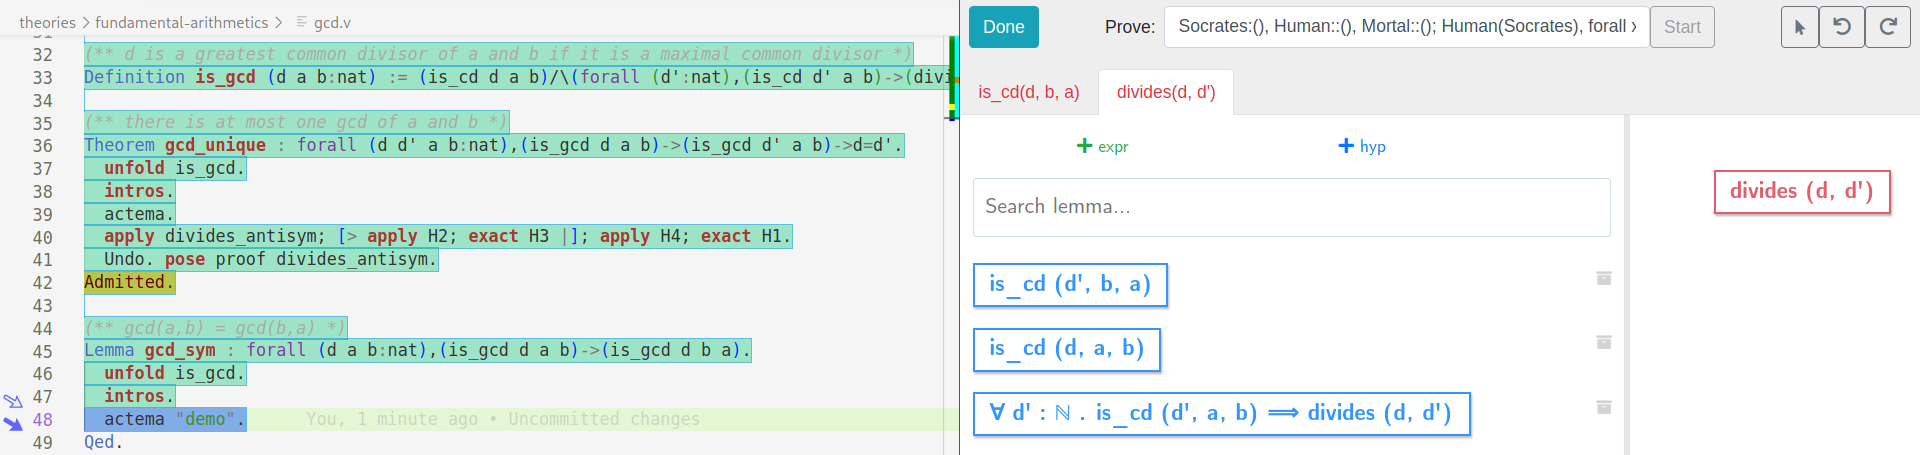
\includegraphics[width=1.5\textwidth]{coq-actema.png}
  \caption{ A possible graphical layout of the \texttt{coq-actema} system. On
    the left, the usual interactive view of the proof script, in the VsCoq IDE.
    On the right, the graphical proof view of Actema.}
  \labfig{coq-actema}
\end{figure*}

\begin{figure*}
  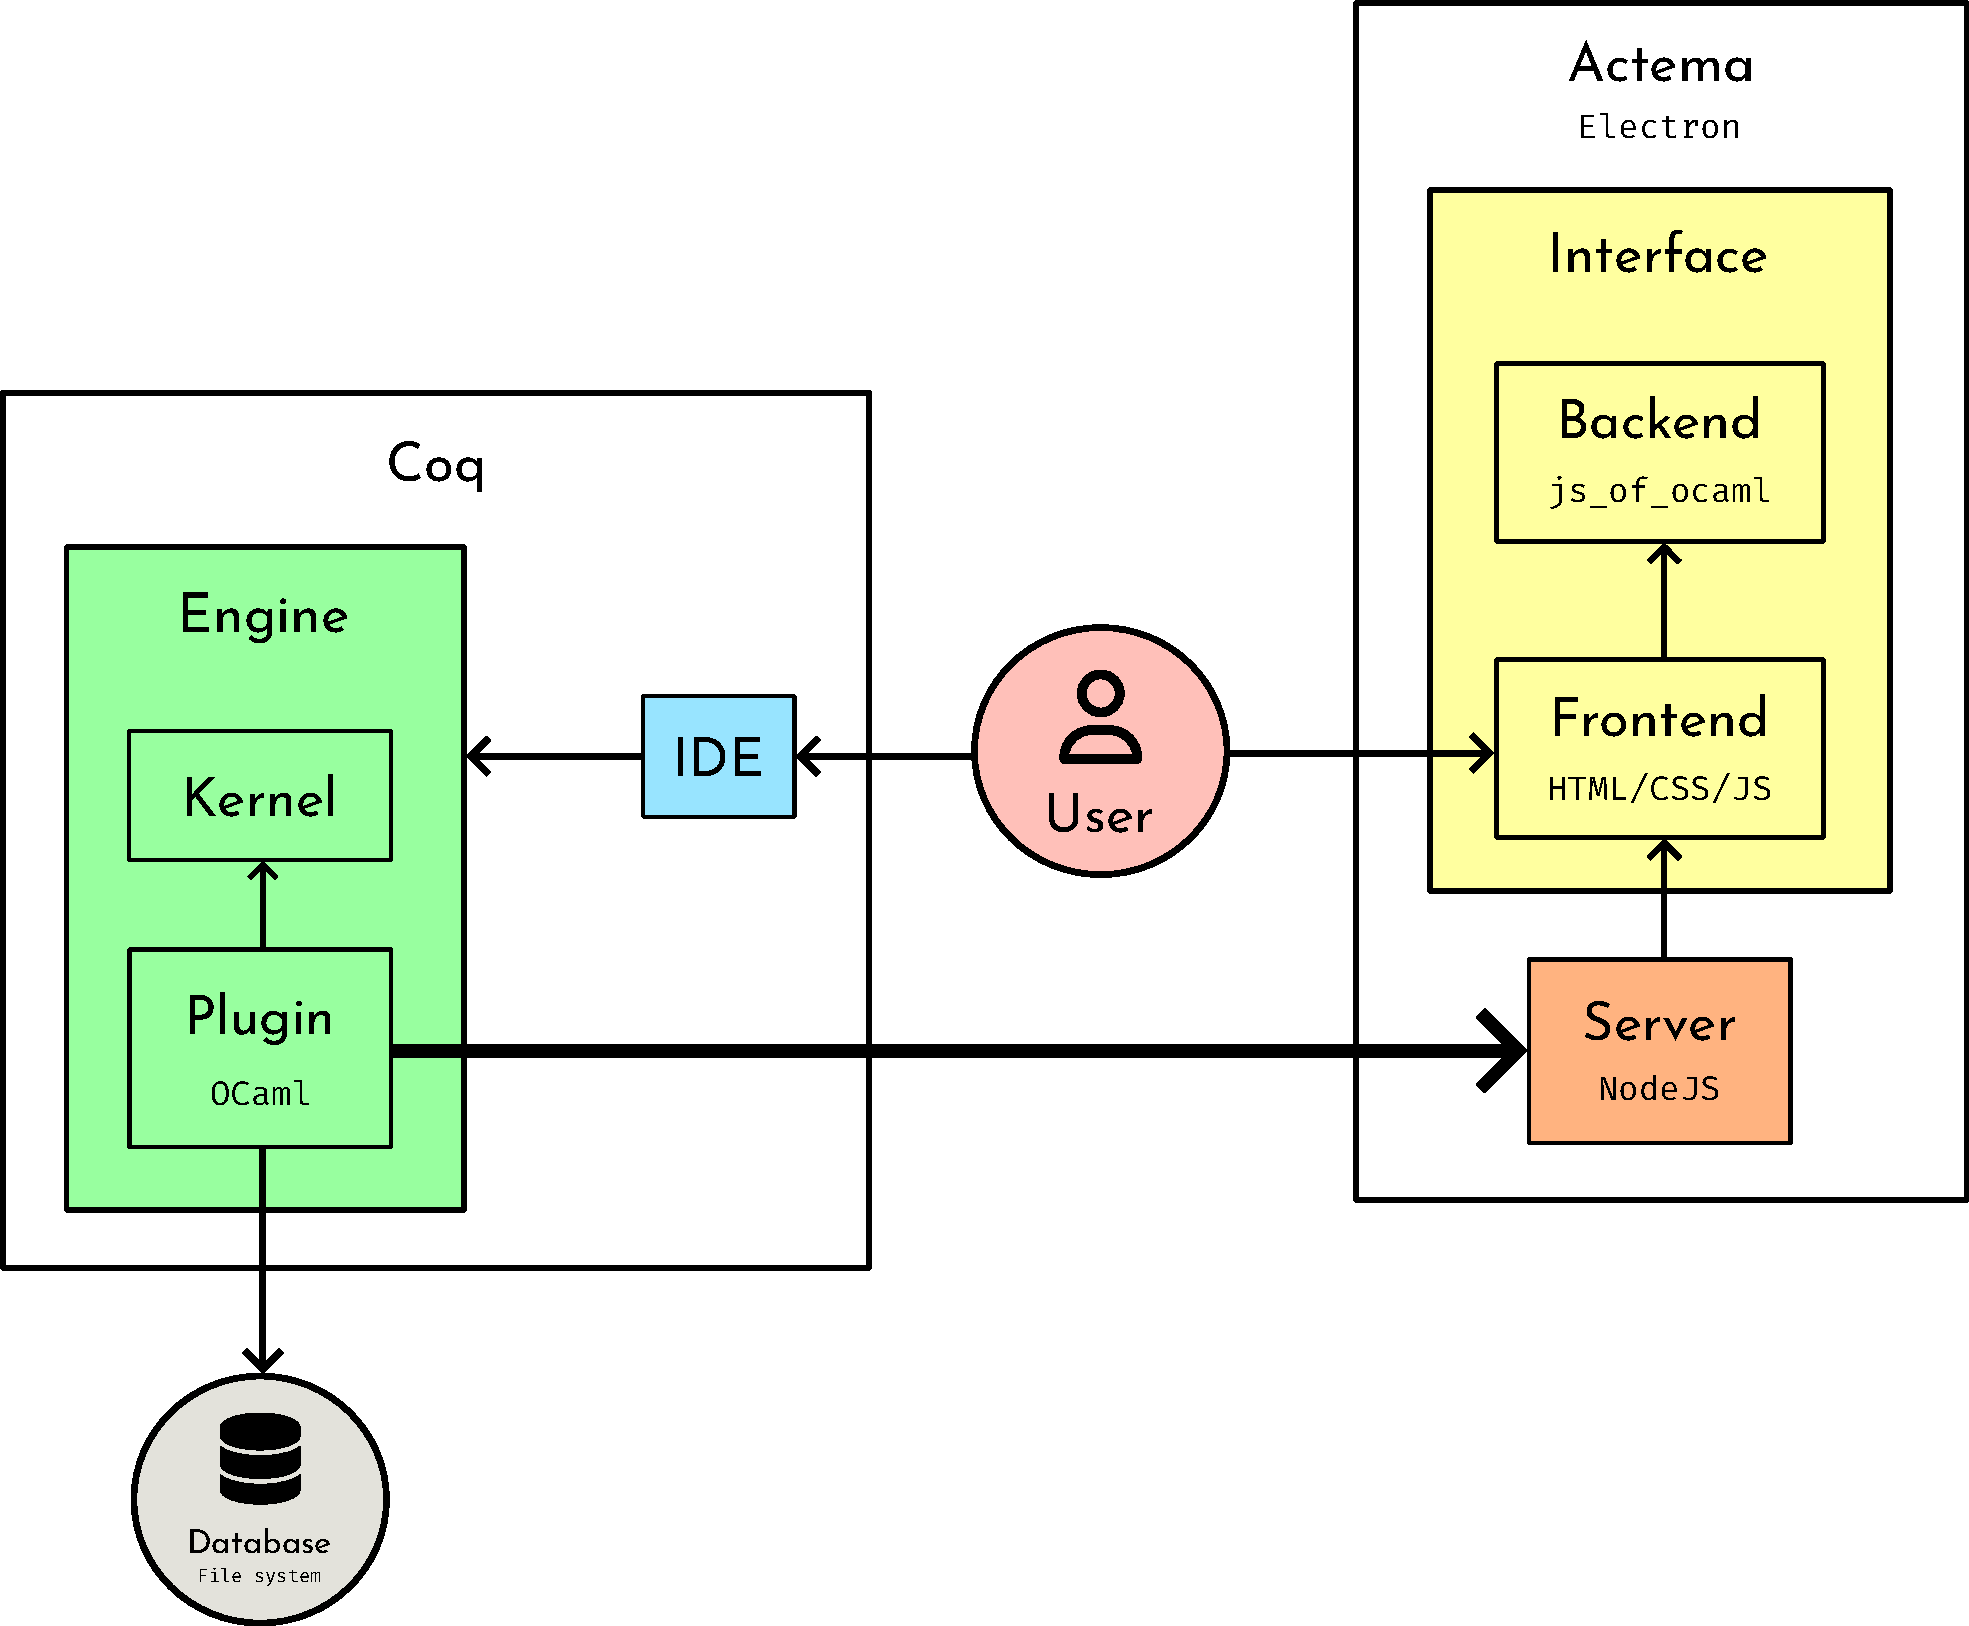
\includegraphics[width=1.3\textwidth]{archi.pdf}
  \caption{Architecture of the \texttt{coq-actema} system}
  \labfig{archi}
\end{figure*}

\todo{ Add link to GitHub repository of coq-actema (which should thus become
  public)}

Let us now give the full picture of the \texttt{coq-actema} system that
integrates both Actema and the Coq plugin. A schematic view of its overall
architecture, including the various components and their relationships, is
provided in \reffig{archi}. The different \emph{processes/agents} involved are
represented by shapes of different \emph{colors}, and we add a directed
\emph{arrow} whenever two of them communicate with each other, where the
\emph{source} requests data from, or sends instructions to the \emph{target}.

The \process{User} (pink circle) is the only human agent in the system, and
drives all interactions. She interacts with the Coq and Actema subsystems
(transparent rectangles), through the interfaces provided by her Coq
\process{IDE} of choice (blue rectangle) and Actema's \process{Frontend} (yellow
rectangle). This will typically take the form of a two-windows layout, as
depicted by the screenshot of \reffig{coq-actema}.

\subsection{Actema web app}

The Actema web app runs in a process independent from Coq, represented by the
yellow \process{Interface} rectangle. We add a third layer to the
\process{Frontend} and \process{Backend} described in \refsec{actema}, namely a
HTTP \process{Server} (orange rectangle) that handles requests from, and
responses to the Coq \process{Plugin}. Thus we implement interprocess
communication between Actema and Coq through the network layer of the operating
system, rather than a more local mechanism such as Unix pipelines. There are a
few reasons behind our choice of the HTTP protocol:
\begin{itemize}
  \item it provides useful abstractions when working with a client/server
    architecture structured around requests;
  \item it is a widely spread standard, especially in web technologies. Thus we
    were able to reduce development time by reusing generic implementations of
    both client and server from standard libraries;
  \item more anecdotically, this makes it easy to run Coq and Actema on
    different machines connected on the same network. This could be used for
    instance to offload heavy computations in a proof to the machine running
    Coq, while still being able to interact with Coq through Actema on the
    weaker machine.
\end{itemize}
The \process{Server} runs in a process separate from the \process{Interface}, in
order to avoid any delay in the latter. Then we bundle everything in an Electron
application \sidecite{Electron}, so that Actema can easily be run locally on
most operating systems. This also allows us to exploit the multi-process
architecture of Electron \sidecite{ElectronProcess}, where the so-called
\emph{main} process runs the server and has the ability to issue system calls
for networking through the Node.js HTTP library \sidecite{NodeJS}; and the
so-called \emph{renderer} process runs the \process{Interface} in the Chromium
browser.

\subsection{Coq plugin}

The \process{Plugin} is loaded dynamically in Coq's \process{Engine} (green
rectangle) by executing the following command in a proof script:
\begin{minted}[fontsize=\normalsize]{coq}
  From Actema Require Import Loader.
\end{minted}
% This can be done dynamically by the \process{User} in her \process{IDE}, or
% statically at compile time.
It essentially exposes a single tactic called \texttt{actema}, which can run in
two distinct modes:
\begin{enumerate}
  \item[\bfseries Interactive] The \process{Plugin} sends the current subgoals
  to Actema, and the user applies a sequence of actions on them. Each time an
  action is performed, it is sent back to Coq, compiled into the appropriate
  tactic call, and then executed to generate new subgoals that are sent again to
  Actema. The \texttt{actema} tactic finishes its execution either when:
  \begin{itemize}
    \item all subgoals are proved (in Actema);
    \item the \process{User} decides to stop and give back control to the
    \process{IDE};
    \item in some rare cases, an unrecoverable error occurs.
  \end{itemize}

  \item[\bfseries Non-interactive] If the \texttt{actema} tactic has already
  been executed on the subgoal under focus, then the \process{Plugin}
  automatically saved the sequence of actions performed by the \process{User} in
  a \process{Database} (gray circle). Currently for ease of development, the
  \process{Database} is implemented as a simple directory on the local
  filesystem, where each file encodes an entry as follows:
  \begin{itemize}
    \item the filename is a hash code that uniquely identifies the goal by both
    its \emph{content}, i.e. the statements of the hypotheses and conclusion,
    and an optional \emph{identifier}, which can be given as argument to the
    tactic in the form of an arbitrary string;
    \item the contents of the file is essentially a Base64 encoding of the data
    specifying each action, whose format will be detailed in
    \refsec{compilation}.
  \end{itemize}
  Then the tactic will load the sequence of actions from the appropriate file,
  recompile it into one big tactic, and execute it on the current subgoal.
\end{enumerate}
One can also force the execution in interactive mode by using a variant of the
tactic named \texttt{actema\_force}. We provide details of the complete
interaction protocol followed by the \texttt{actema} tactic in the following
section.

Regarding the implementation of the \process{Plugin}, we chose to do it in the
standard way by interfacing with the \texttt{coq-core} API in OCaml
\sidecite{CoqCore}, although it has been encouraged in recent versions of Coq to
interface with more stable APIs such as those provided by Coq-Elpi
\sidecite{CoqELPI} and MetaCoq \sidecite{MetaCoq}\sidenote{Indeed breaking
changes are frequently introduced in \texttt{coq-core} with newer versions of
Coq, which requires more maintenance efforts from plugin developers.}. The main
reason is that our plugin performs \emph{side effects} by interacting with an
external environment: the file system when saving and retrieving graphical
proofs, and the network when issueing HTTP requests to Actema. Those cannot be
implemented in the aforementioned frameworks, and in fact are not part of the
\texttt{coq-core} API either.

\section{Interaction protocol}\labsec{protocol}

\section{Compiling actions}\labsec{compilation}

\section{Future works}\labsec{pluginfuture}

\begin{itemize}
  \item Switch to \emph{higher-order logic} in Actema's backend
  \item Extend HTTP protocol to support \emph{lemma search}
  \item Display goal with Coq \emph{notations} (or develop a framework for
    \emph{interactive} notations in the style of ProofWidgets)
  \item Individual translation of actions to reusable tactic calls
  \item Replay mode
\end{itemize}